\section{Auswahl der Skriptsprachen}
\setauthor{Robert Freiseisen}

Die Wahl der Scriptsprachen wurde auf Grund einer intensiven Internet-Recherchen 
und Fachgesprächen mit Mitschüler*innen und Professor*innen gefällt.\\
Folgende Scriptsprachen wurden gewählt:

\subsection{Lua}
Lua ist eine extrem schnelle Programmiersprache, die für ihre hohe Ausführungsgeschwindigkeit geschätzt wird. 
Diese Schnelligkeit, kombiniert mit dem geringen Speicherbedarf der Sprache, macht sie ideal für ressourcenbeschränkte Umgebungen und eingebettete Systeme. 
Lua bietet eine "Out-of-the-Box"-Nutzbarkeit, die es Entwicklern ermöglicht, sofort nach der Installation loszulegen, ohne sich um eine Vielzahl von Abhängigkeiten kümmern zu müssen. 
Ihre Einbettbarkeit ist ein weiteres Kernelement, das sie besonders attraktiv für Softwareprojekte macht, die eine integrierte Skriptsprache benötigen. Besonders in der Spieleindustrie hat Lua sich als beliebte Wahl für das Scripting etabliert. Hier ermöglicht es Entwicklern, schnell interaktive und flexible Spielmechanismen zu implementieren, ohne die Hauptspiellogik zu beeinträchtigen. 
Als Open-Source-Software steht Lua zudem einer breiten Entwicklergemeinschaft zur Verfügung, die zur kontinuierlichen Verbesserung und Erweiterung der Sprache beiträgt.
All diese Aspekte machen Lua zu einer vielseitigen und kraftvollen Option für eine Reihe von Anwendungen, insbesondere für das Scripting in Videospielen, wie in "World of Warcraft" oder "Roblox".

\newpage
\subsection{IronPython}
IronPython ist eine Implementierung der Python-Programmiersprache, die auf dem .NET-Framework aufbaut, nicht auf der Java Virtual Machine (JVM). 
In Bezug auf Schnelligkeit kann IronPython, je nach Anwendungsfall, sowohl Vorteile als auch Nachteile gegenüber der standardmäßigen CPython-Implementierung haben. 
Da es auf dem .NET Framework basiert, kann es schneller sein, wenn es darum geht, mit anderen .NET-Anwendungen oder Bibliotheken zu interagieren. 
Beim Speicherverbrauch ist IronPython in der Regel nicht so effizient wie CPython, da das .NET-Framework mehr Overhead haben kann. 
Einer der größten Vorteile von IronPython ist seine Dynamik. 
Durch die Nutzung der Dynamic Language Runtime (DLR) von .NET kann IronPython dynamische Typen und späte Bindungen effizienter verwalten als einige andere Implementierungen. 
Dies ermöglicht eine enge Integration mit .NET-Bibliotheken und erleichtert die schnelle Entwicklung und Iteration von Code.

\newpage
\subsection{Csharpscript}
CSharpScript ist eine Bibliothek, die die Ausführung von Csharp-Skripten ermöglicht, und stellt eine flexible Möglichkeit dar, Csharp-Code dynamisch auszuführen. 
Einer der großen Vorteile von CSharpScript ist, dass es sowohl in gehosteten als auch in eigenständigen Ausführungsmodellen eingesetzt werden kann. 
In einem gehosteten Modell kann das Skript innerhalb einer bestehenden Anwendung laufen und Objekte und Funktionen der Anwendung nutzen oder modifizieren. 
In einem eigenständigen Modell kann das Skript als unabhängige Anwendung ausgeführt werden. 
Ein weiteres wichtiges Merkmal ist die Kompatibilität mit .NET 5/Core und höheren Versionen. 
Dies ermöglicht eine bessere Leistung, erweiterte APIs und die Möglichkeit, plattformübergreifende Anwendungen zu entwickeln. 
Die Bibliothek stellt eine robuste Schnittstelle bereit, die die Integration von Csharp-Skripten in eine Vielzahl von Anwendungsdomänen vereinfacht.


\newpage
\subsection{Javascript}
JavaScript ist eine äußerst populäre und vielseitige Programmiersprache, die vor allem in der Webentwicklung eingesetzt wird. 
Sie zeichnet sich durch ihre Einfachheit und Benutzerfreundlichkeit aus, was sie besonders für Einsteiger attraktiv macht. 
Die Sprache ist intuitiv aufgebaut, sodass die grundlegenden Konzepte schnell verstanden und angewendet werden können. 
Ein weiterer Vorteil ist, dass alle modernen Webbrowser eine JavaScript-Engine integriert haben. 
Dies ermöglicht es Entwicklern, Code unmittelbar im Browser auszuführen und zu testen, ohne zusätzliche Software installieren zu müssen. 
In Bezug auf die Sicherheit bietet JavaScript zwar einige Mechanismen, wie die Ausführung in einer Sandbox-Umgebung, um den Zugriff auf das Betriebssystem des Nutzers zu beschränken. 
Allerdings ist es wichtig, die Risiken von Cross-Site-Scripting (XSS) zu berücksichtigen, einer Art von Angriff, der durch schlecht geschützte JavaScript-Code ermöglicht wird. 
Daher ist es essentiell, bewährte Sicherheitspraktiken anzuwenden, um solche Schwachstellen zu minimieren. 
Insgesamt bietet JavaScript eine ausgewogene Mischung aus Benutzerfreundlichkeit, Intuitivität und Funktionalität, allerdings müssen Entwickler stets wachsam in Bezug auf Sicherheitsrisiken wie XSS sein.

\newpage
\section{Kriterienkatalog}
\setauthor{Robert Freiseisen}
Jede der untersuchten Sprachen hat ihre eigenen Vor- und Nachteile, und die Auswahl der besten Option kann je nach Projektanforderungen variieren. 
In diesem Abschnitt betrachten wir diese vier Sprachen im Kontext von .NET unter verschiedenen Aspekten:

\begin{itemize}
    \item Aktivität der Entwicklung: 
    \begin{itemize}
        \item Wie lebendig und aktiv ist die Community hinter der Sprache? 
        \item Wie oft werden Updates veröffentlicht, und wie gut ist die Dokumentation?
    \end{itemize}
    \item Funktionalität:
    \begin{itemize}
        \item Welche Features bietet die Sprache, und wie reichhaltig ist ihr Ökosystem? 
        \item Gibt es umfangreiche Bibliotheken, die die Entwicklung erleichtern?
    \end{itemize}
    \item Einsetzbarkeit:
    \begin{itemize}
        \item Wie einfach lässt sich die Sprache in bestehende oder neue .NET-Projekte integrieren?
        \item Welche Voraussetzungen müssen erfüllt sein, und wie komplex ist die Integration?
    \end{itemize}
    \item Performance:
    \begin{itemize}
        \item Wie steht es um die Laufzeit-Performance des Codes? 
        \item  Inwiefern beeinflusst die Wahl der Sprache die Geschwindigkeit und Ressourceneffizienz der fertigen Anwendung?
    \end{itemize}
    \item Debugging:
    \begin{itemize}
        \item Welche Möglichkeiten bietet die Sprache für das Debugging von Code?
        \item Wie effektiv lassen sich Fehler finden und beheben, und welche Werkzeuge stehen zur Verfügung?
    \end{itemize}
\end{itemize}

\newpage
Alle Daten wurden auf zwei unterschiedlichen Geräten gemessen. \\
Die Daten für IronPython und Lua wurden auf \\
PC A unter folgenden Voraussetzungen  gemessen:
\begin{itemize}
    \item Gerätspezifikationen:
    \begin{table}[H]
        \center
        \begin{tabular}{|p{3cm}|p{3cm}|}
            \hline
            Hersteller & HP \\ \hline
            Gerätname & LAPTOP-5U1879KR \\ \hline
            Prozessor & Intel(R) Core(TM) i5-8265U CPU @ 1.60GHz   1.80 GHz \\ \hline
            Installierter RAM & 8.00 GB (7.89 GB verwendbar) \\ \hline
            Produkt-ID & 00325-81357-65742-AAOEM \\ \hline
            Systemtyp & 64-Bit-Betriebssystem, x64-basierter Prozessor \\ \hline
        \end{tabular}
    \end{table}
    \item Betriebssystem:
    \begin{table}[H]
        \center
        \begin{tabular}{|p{4cm}|p{4cm}|}
            \hline
            Edition & Windows 11 Home \\ \hline
            Version & 21H2 \\ \hline
            Installiert am & 24.11.2021 \\ \hline
            Betriebssystembuild & 220.001.098 \\ \hline
            Leistung & Windows Feature Experience Pack 1000.22000.1098.0 \\ \hline
        \end{tabular}        
    \end{table}
\end{itemize}

\newpage
Die Daten für Csharpscript und Javascript wurden auf \\
PC B unter folgenden Voraussetzungen  gemessen:
\begin{itemize}
    \item Gerätspezifikationen:
    \begin{table}[H]
        \center
        \begin{tabular}{|p{3cm}|p{3cm}|}
            \hline
            Hersteller & Acer \\ \hline
            Gerätname & Beptop \\ \hline
            Prozessor & Intel(R) Core(TM) i5-8265U CPU @ 1.60GHz \\ \hline
            Installierter RAM & 16.00 GB (15.9 GB verwendbar) \\ \hline
            Produkt-ID & C125C288-8DFB-4042-A3BA-EE3236D35AB7 \\ \hline
            Systemtyp & 64-Bit-Betriebssystem, x64-basierter Prozessor \\ \hline
        \end{tabular}
    \end{table}
    \item Betriebssystem:
    \begin{table}[H]
        \center
        \begin{tabular}{|p{4cm}|p{4cm}|}
            \hline
            Edition & Windows 11 Home \\ \hline
            Version & 21H2 \\ \hline
            Installiert am & 06.10.2021 \\ \hline
            Betriebssystembuild & 220.001.098 \\ \hline
            Leistung & Windows Feature Experience Pack 1000.22000.1098.0 \\ \hline
        \end{tabular}        
    \end{table}
\end{itemize}


\newpage
\subsection{Aktivität der Entwicklung}

In der nachfolgenden Tabelle wird dargestellt, wie intensiv die Entwicklerteams an den unterschiedlichen Scriptsprachen arbeiten und ob diese auch die Nuget-Pakete entwickeln.
\begin{table}[H]
    \begin{tabular}{|p{3cm}|p{3cm}|p{3cm}|p{3cm}|p{3cm}|}
        \hline
        Aktivität & IronPython & Lua & CsharpScripting & Javascript\\ \hline
        Commits in den letzten 10 Monaten & 179 & 27 & 702 & 1153 \\ \hline
        Nuget-Packages vom Sprach-entwicklerteam selber &Nein &Nein &Ja & Nein\\ \hline
        Releases in den letzten 10 Monaten & 2 (2.7.1 und 3.4.0-beta1) & 1 (v5.4.4) & v4.0.0 und höher & v4.6.2 (und höher)\\ \hline
        Unterstützt aktuelle major Versionen von Scriptsprache & Ja & Ja & Ja & Ja\\ \hline
        Unterstützt aktuelle Versionen von .NET & Ja & Ja & Ja & Ja \\ \hline
    \end{tabular}
\end{table}
\newpage
\subsection{Einsetzbarkeit}
Die folgende Tabelle stellt dar, auf welchen Betriebssystemen die veschiedenen Scriptsprachen mit .NET lauffähig sind.

\begin{table}[H]
    \center
    \begin{tabular}{|p{3cm}|p{3cm}|p{3cm}|p{3cm}|p{3cm}|}
        \hline
        Einsetzbarkeit & IronPython & Lua & CsharpScripting & Javascript\\ \hline
        Auf Windows lauffähig & Ja & Ja & Ja & Ja \\ \hline
        Auf MAC lauffähig & Ja & Ja & Ja & Ja \\ \hline
        Auf Linux lauffähig & Ja & Ja & Ja & Ja \\ \hline
 
    \end{tabular}
\end{table}
\newpage
\subsection{Performance}
Der Speicherplatzt wurde aus dem Windows-File-Explorer entnommen. 
Die Geschwindigkeitsmessungen erfolgten mit Dotnet-Benchmark.

DotNetBenchmark ist nicht eine standardisierte Bibliothek oder ein offizielles Werkzeug, aber der Begriff könnte in der Kontext von .NET-Entwicklung für Benchmarking-Tests verwendet werden. In der Regel wird BenchmarkDotNet als die vorherrschende Bibliothek für das Benchmarking in der .NET-Umgebung angesehen. Es ermöglicht Entwicklern, die Leistung von .NET-Code einfach und genau zu messen. 
Mit BenchmarkDotNet können Microbenchmarks durchgeführt werden, die sehr spezifische Aspekte des Codes testen, wie zum Beispiel die Ausführungszeit einer Methode.
Als eine einfache Anwendung wird ein Programm genommen, dass eine Funktion aufruft, welche 42 zurück gibt 
und dies anschließen auf die Konsole ausgibt.
\begin{table}[H]
    \begin{tabular}{|p{3cm}|p{3cm}|p{3cm}|p{3cm}|p{3cm}|}
        \hline
        Performance & IronPython & Lua & CsharpScripting & Javascript\\ \hline
        Speicher einer einfachen Anwendung & 13 MB & 7.3 MB & 168 KB & 416 KB  \\ \hline
        Durchnittliche Laufzeit einer einfachen Anwendung & 137.118 $\mu$s & 8.088 $\mu$s & 90.24 $\mu$s & 31.65 $\mu$s \\ \hline
        Durchnittliche Laufzeit einer Additionsfunktion & 2340.688 $\mu$s & 10.053 $\mu$s & 83.82 $\mu$s & 16.03 $\mu$s \\ \hline
        Durchnittliche Laufzeit von Übergabe eines .NET-Objekts & 9054.007 $\mu$s & 7548.497 $\mu$s &  & \\ \hline
    \end{tabular}
\end{table}

\newpage
Es folgen nun die Resultate von Dotnet-Benchmark:
\linebreak
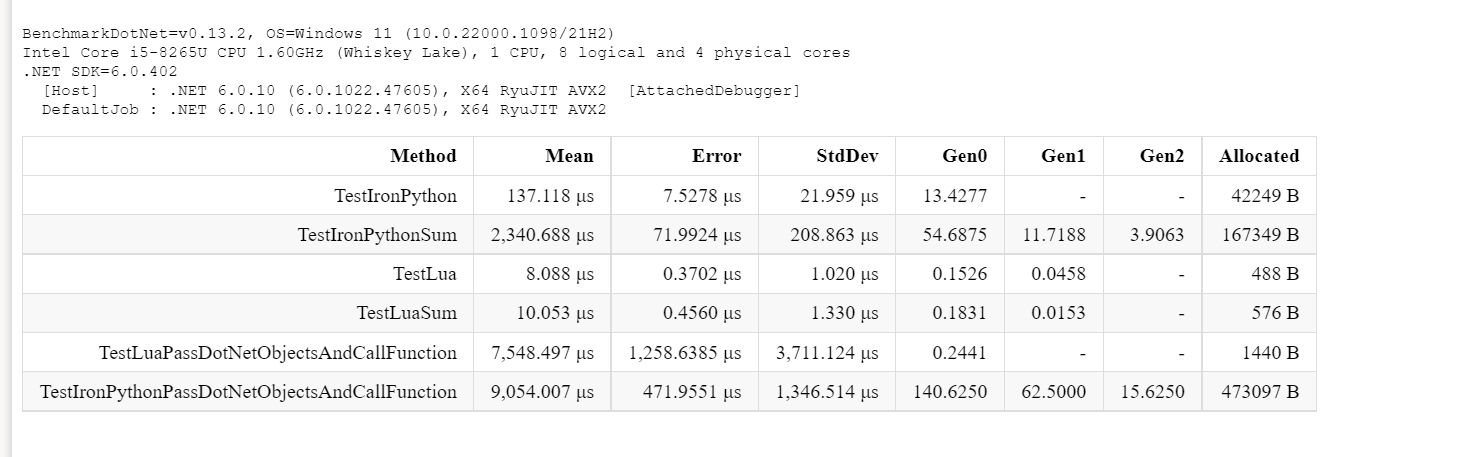
\includegraphics[scale=0.5]{pics/benchmark_results_NluaVsIronPython.png}
\newpage
\subsection{Funktionalität}
In der nachfolgenden Tabelle sind die Recherche-Ergebnisse hinsichtlich der Funktionalität der Scriptsprachen in .NET dargestellt.
Die Informationen wurden aus den offizellen Webseiten der Nuget-Pakete entnommen.

\begin{table}[H]
    \begin{tabular}{|p{3cm}|p{3cm}|p{3cm}|p{3cm}|p{3cm}|}
        \hline
        Funktion & IronPython & Lua & CsharpScripting & Javascript\\ \hline
        Kann auf .NET Variablen zugreifen & Ja & Ja & Ja & Ja \\ \hline
        Kann globale Variablen & Ja & Ja & Ja & Ja \\ \hline
        Unterstützt Erweiterungspakete der Scriptsprache & Ja (nicht numpy und pandas!) & Ja & Ja & Ja \\ \hline 
    \end{tabular} 
\end{table}
\newpage
\subsection{Debugging}
In der nachfolgenden Tabelle ist dargestellt, welche Art des Debugging bei welcher Scriptsprache möglich ist.

\begin{table}[H]
    \begin{tabular}{|p{2.5cm}|p{2.5cm}|p{2.5cm}|p{2.5cm}|p{2.5cm}|}
        \hline
        Debugging & IronPython & Lua & CsharpScripting & Javascript\\ \hline
        Debugging durch Ausgabe auf der Konsole & Ja & Ja & Ja & Ja \\ \hline
        Debugging mit Break Points in Visual Studio & Ja & Nein & Nein & Nein\\ \hline
        Debugging mit Break Points in Visual Studio Code & Ja & Nein & Nein & Nein \\ \hline
    \end{tabular}
\end{table}